\documentclass[aspectratio=169,compress,mathserif]{beamer}
\usepackage{tikz}

\newcommand{\regressiontable}[1]{\begin{tabular}{lcccc} \hline \hline
 & (1) & (2) & (3) & (4) \\
		& \begin{tabular}[x]{@{}c@{}}lnL\end{tabular}
		& \begin{tabular}[x]{@{}c@{}}lnKL\end{tabular}
		& \begin{tabular}[x]{@{}c@{}}lnQL\end{tabular}
		& \begin{tabular}[x]{@{}c@{}}exporter\end{tabular}   \\ \hline
 & & & &   \\
	\begin{tabular}[x]{l}Foreign owner (dummy)\end{tabular}
			&  \begin{tabular}[x]{@{}c@{}}0.401${}^*$${}^*$${}^*$
			 \\ (0.021)\end{tabular}
			&  \begin{tabular}[x]{@{}c@{}}0.602${}^*$${}^*$${}^*$
			 \\ (0.032)\end{tabular}
			&  \begin{tabular}[x]{@{}c@{}}0.664${}^*$${}^*$${}^*$
			 \\ (0.023)\end{tabular}
			&  \begin{tabular}[x]{@{}c@{}}0.350${}^*$${}^*$${}^*$
			 \\ (0.007)\end{tabular} \\
	\begin{tabular}[x]{l}Expat manager (dummy)\end{tabular}
			&  \begin{tabular}[x]{@{}c@{}}0.016
			 \\ (0.025)\end{tabular}
			&  \begin{tabular}[x]{@{}c@{}}0.073${}^*$
			 \\ (0.041)\end{tabular}
			&  \begin{tabular}[x]{@{}c@{}}-0.076${}^*$${}^*$${}^*$
			 \\ (0.028)\end{tabular}
			&  \begin{tabular}[x]{@{}c@{}}0.050${}^*$${}^*$${}^*$
			 \\ (0.008)\end{tabular} \\
\\
	$R^2$ 
				& 0.069 
				& 0.166 
				& 0.235 
				& 0.190 \\
	Number of observations 
				& 368,493 
				& 368,493 
				& 368,493 
				& 368,493 \\
\hline \hline
\multicolumn{ 5 }{c}{\begin{minipage}{\textwidth}
\small Notes: All specifications control for industry-year fixed effects and firm age. Standard errors, clustered by firm, are reported in parantheses. Coefficients significantly different from zero at 1, 5 and 10 percent are marked by ***, ** and *, respectively.

  \end{minipage} } \\
\end{tabular}}

\newcommand{\scaffolding}{\draw [->] (0,-0.5) --(14,-0.5);
\draw[thick] (7,-0.5)--(10,-0.5);

\foreach \x in {1,4,7,10,13}
\draw(\x cm,3pt - 0.5cm) -- (\x cm, -3pt - 0.5cm);
}
%\usepackage[absolute]{textpos}
%\documentclass[handout,compress,mathserif]{beamer}
%\setbeameroption{show notes}

% This file is a solution template for:

% - Talk at a conference/colloquium.
% - Talk length is about 20min.
% - Style is ornate.



% Copyright 2004 by Till Tantau <tantau@users.sourceforge.net>.
%
% In principle, this file can be redistributed and/or modified under
% the terms of the GNU Public License, version 2.
%
% However, this file is supposed to be a template to be modified
% for your own needs. For this reason, if you use this file as a
% template and not specifically distribute it as part of a another
% package/program, I grant the extra permission to freely copy and
% modify this file as you see fit and even to delete this copyright
% notice.


\mode<presentation>
{
%  \usetheme{pittsburgh}
  % or ...

  \setbeamercovered{invisible}
  % or whatever (possibly just delete it)
}


\usepackage[utf8]{inputenc}


\renewcommand{\cite}[1]{({\small #1})}

\pretolerance5000 \hyphenpenalty9999
%\setlength{\TPHorizModule}{0.5cm} \setlength{\TPVertModule}{0.5cm}
%\textblockorigin{20mm}{20mm} % start everything near the top-left corner

\newcounter{ora}
\newcounter{perc}
\newcounter{kezdoora}
\newcounter{kezdoperc}
\newcounter{percek}
\setcounter{percek}{15}
\setcounter{kezdoora}{4} % for 1.35pm as the starting time

\providecommand{\leadingzero}[1]{\ifthenelse{\value{#1}<10}{0\arabic{#1}}{\arabic{#1}}}
\providecommand{\oradisplay}[1]{\ifthenelse{\value{#1}<60}{\arabic{kezdoora}:\leadingzero{#1}}{\setcounter{perc}{\value{#1}}\addtocounter{perc}{-60}\setcounter{ora}{\value{kezdoora}}\addtocounter{ora}{1}\arabic{ora}:\leadingzero{perc}}}

\providecommand{\notes}[1]{{\tiny\textbf{Note:} #1}}
%%%%%%%%%%%%%%%%%%%%%%%%%%%%%%%%%%%%%%%%%%%%%%%%
%% Hasznos matek makrok
%%%%%%%%%%%%%%%%%%%%%%%%%%%%%%%%%%%%%%%%%%%%%%%%

\newcommand{\QED}{{}\hfill$\Box$}
\newcommand{\intl}[4]{\int_{#1}^{#2} \! {#3} \, \mathrm d{#4}}
\newcommand{\period}{\text{.}} % Ez azert kell, mert a matek . mashogy nez ki, mint a szovege.
\newcommand{\comma}{\text{,}}  % Ez azert kell, mert a matek , mashogy nez ki, mint a szovege.
\newcommand{\dist}{\,\mathop{\operatorname{\sim\,}}\limits}
\newcommand{\D}{\,\mathop{\operatorname{d}}\!}
%\newcommand{\E}{\mathop{\operatorname{E}}\nolimits}
\newcommand{\Lag}{\mathop{\operatorname{L}}}
\newcommand{\plim}{\mathop{\operatorname{plim}}\limits_{T\to\infty}\,}
\newcommand{\CES}[3]{\mathop{\operatorname{CES}}\left(\left\{#1\right\},\left\{#2\right\},#3\right)}
\newcommand{\cestwo}[5]{\left[#1^\frac1{#5}\,#2^\frac{#5-1}{#5}+#3^\frac1{#5}\,#4^\frac{#5-1}{#5}\right]^\frac{#5}{#5-1}}
\newcommand{\cesmore}[4]{\left[\sum_{#3}#1_{#3}^\frac1{#4}\,{#2}_{#3}^\frac{#4-1}{#4}\right]^\frac{#4}{#4-1}}
\newcommand{\cesPtwo}[5]{\left[#1\,#2^{1-#5}+#3\,#4^{1-#5}\right]^\frac{1}{1-#5}}
\newcommand{\cesPmore}[4]{\left[\sum_{#3}#1_{#3}\,#2_{#3}^{1-#4}\right]^\frac{1}{1-#4}}
\newcommand{\diff}[2]{\frac{\D #1}{\D #2}}
\newcommand{\pdiff}[2]{\frac{\partial #1}{\partial #2}}
\newcommand{\convex}[2]{\lambda #1 + (1-\lambda)#2}
\newcommand{\ABS}[1]{\left| #1 \right|}
\newcommand{\suchthat}{:\hskip1em}
\newcommand{\dispfrac}[2]{\frac{\displaystyle #1}{\displaystyle #2}} % Emeletes tortekhez hasznos.

\newcommand{\diag}{\mathop{\mathrm{diag\mathstrut}}}
\newcommand{\tr}{\mathop{\mathrm{tr\mathstrut}}}
\newcommand{\E}{\mathop{\mathrm{E\mathstrut}}}
\newcommand{\Var}{\mathop{\mathrm{Var\mathstrut}}\nolimits}
\newcommand{\Cov}{\mathop{\mathrm{Cov\mathstrut}}}
\newcommand{\sgn}{\mathop{\operatorname{sgn\mathstrut}}}

\newcommand{\covmat}{\mathbf\Sigma}
\newcommand{\ones}{\mathbf 1}
\newcommand{\zeros}{\mathbf 0}
\newcommand{\BAR}[1]{\overline{#1}}

\renewcommand{\time}[1]{\addtocounter{percek}{#1}}

\newlength{\tempsep}

\newenvironment{subeqs}{\setlength{\tempsep}{\arraycolsep}
\setlength{\arraycolsep}{0.13889em} % Ez azert kell, hogy ne hagyjon tul sok helyet az = korul.
\begin{subequations}\begin{eqnarray}}
{\end{eqnarray}\end{subequations}
\setlength{\arraycolsep}{\tempsep}}

\newenvironment{tapad}{\setlength{\tempsep}{\arraycolsep}
\setlength{\arraycolsep}{0.13889em}} % Ez azert kell, hogy ne hagyjon tul sok helyet az = korul.
{\setlength{\arraycolsep}{\tempsep}}

\newenvironment{eqnarr}{\setlength{\tempsep}{\arraycolsep}
\setlength{\arraycolsep}{0.13889em} % Ez azert kell, hogy ne hagyjon tul sok helyet az = korul.
\begin{eqnarray}}
{\end{eqnarray} \setlength{\arraycolsep}{\tempsep}}

\newenvironment{eqnarr*}{\setlength{\tempsep}{\arraycolsep}
\setlength{\arraycolsep}{0.13889em} % Ez azert kell, hogy ne hagyjon tul sok helyet az = korul.
\begin{eqnarray*}}
{\end{eqnarray*} \setlength{\arraycolsep}{\tempsep}}


%\usepackage[active]{srcltx} % SRC Specials: DVI [Inverse] Search
% Fuzz --- -------------------------------------------------------
\hfuzz5pt % Don't bother to report over-full boxes < 5pt
\vfuzz5pt % Don't bother to report over-full boxes < 5pt
% THEOREMS -------------------------------------------------------
% MATH -----------------------------------------------------------
\newcommand{\norm}[1]{\left\Vert#1\right\Vert}
\newcommand{\abs}[1]{\left\vert#1\right\vert}
\newcommand{\set}[1]{\left\{#1\right\}}
\newcommand{\Real}{\mathbb R}
\newcommand{\eps}{\varepsilon}
\newcommand{\To}{\longrightarrow}
\newcommand{\BX}{\mathbf{B}(X)}
\newcommand{\A}{\mathcal{A}}




\newcommand{\directory}{output/figure}
\newcommand*{\newtitle}{\egroup\begin{frame}\frametitle}

\newcommand{\fullpagefigure}[2]{\begin{frame}\frametitle{\hyperlink{#1back}{#2}}\hypertarget{#1}{{\begin{center}\includegraphics[height=0.9\textheight]{\directory/#1}\end{center}}}\end{frame}}
\newcommand{\widefigure}[2]{\begin{frame}\frametitle{\hyperlink{#1back}{#2}}\hypertarget{#1}{{\begin{center}\includegraphics[width=\linewidth]{\directory/#1}\end{center}}}\end{frame}}
\newcommand{\longfigure}[2]{\begin{frame}\frametitle{\hyperlink{#1back}{#2}}\hypertarget{#1}{{\begin{center}\includegraphics[height=0.8\textheight]{\directory/#1}\end{center}}}\end{frame}}
%\newcommand{\fullpagefigure}[2]{\begin{frame}\frametitle{\hyperlink{#1back}{#2}}\hypertarget{#1}{{\begin{centering}$#1$\end{centering}}}\end{frame}}
\newcommand{\answer}[1]{\begin{itemize}\item #1\end{itemize}}


\newcommand{\jumpto}[2]{\hypertarget{#1back}{\hyperlink{#1}{#2}}}
\newcommand{\backto}[2]{\hypertarget{#1}{\hyperlink{#1back}{#2}}}


\title{Expatriate Managers and Firm Performance}

\author{Miklós Koren\\
CEU, MTA KRTK and CEPR\\
Álmos Telegdy\\
MNB and MTA KRTK}
% - Give the names in the same order as the appear in the paper.
% - Use the \inst{?} command only if the authors have different
%   affiliation.


\date % (optional, should be abbreviation of conference name)
{Thanks: ERC Knowledgeflows\\Krisztián Fekete, Olivér Kiss, Szilárd Perédi,\\ Bálint Szilágyi, András Vereckei, Rita Zágoni, Gergő Závecz}
% - Either use conference name or its abbreviation.
% - Not really informative to the audience, more for people (including
%   yourself) who are reading the slides online

%\subject{Theoretical Computer Science}
% This is only inserted into the PDF information catalog. Can be left
% out.



% If you have a file called "university-logo-filename.xxx", where xxx
% is a graphic format that can be processed by latex or pdflatex,
% resp., then you can add a logo as follows:

\logo{}



% Delete this, if you do not want the table of contents to pop up at
% the beginning of each subsection:
\AtBeginSection[]
{
  \begin{frame}[plain]
    \frametitle{\color{red}\insertsection}
    \addtocounter{framenumber}{-1}
    %\tableofcontents[currentsection,currentsubsection]
  \end{frame}
}


% If you wish to uncover everything in a step-wise fashion, uncomment
% the following command:

%\beamerdefaultoverlayspecification{<+->}

\setbeamertemplate{navigation symbols}{}
\setbeamertemplate{footline}{{}\hfill\insertframenumber}

\begin{document}

\begin{frame}[plain]
  \titlepage
    \addtocounter{framenumber}{-1}
\end{frame}






\section{Motivation}\hypertarget{Motivation}{}
\begin{frame}\frametitle{Motivation}\hypertarget{Motivation}{}
\begin{itemize}
\item Some firms produce vastly more output per worker than others (Syverson, 2011).
\begin{itemize}
\item technology

\item organization

\item unmeasured input quality




\end{itemize}

\end{itemize}
\end{frame}



\begin{frame}\frametitle{Management improves firm performance}\hypertarget{Management improves firm performance}{}
\begin{itemize}
\item Good management practices  increase  productivity  (Bloom  and  Van  Reenen  2010;  Bloom  et  al.  2012;  Bloom  et  al.  2014) and market access (Bloom et al. 2016). 

\item CEOs behaving like ``leaders" gradually improve firm performance. (Bandiera, Hansen, Prat and Sadun 2018)

\item Large increase  in  the  level  and  inequality  of  CEO  pay.  (Murphy  and  Zábojník  2004;  Gabaix  and  Landier  2008;  Tervio  2008; Frydman and Saks 2010)


\end{itemize}
\end{frame}



\begin{frame}\frametitle{Manager identity matters}\hypertarget{Manager identity matters}{}
\begin{itemize}
\item Managers have persistent effects across firms on investment policy, R\&D, advertising, return on assets.  (Bertrand and Schoar 2003)

\item Sudden CEO death worsens firm performance. (Bennedsen, Pérez-González and Wolfenzon 2007) 

\item Managers having past export experience increase likelihood of exporting (Mion and Opromolla 2014; Mion, Opromolla and Sforza 2016) and importing (Bisztray, Koren and Szeidl 2018).


\end{itemize}
\end{frame}



\begin{frame}\frametitle{Foreign owned firms perform better than domestic firms}\hypertarget{Foreign owned firms perform better than domestic firms}{}
\begin{itemize}
\item US: Doms and Jensen (1998)

\item UK: Griffith (1999)

\item Hungary, Romania, Russia, Ukraine: Brown, Earle, Telegdy (2006)

\item Indonesia: Arnold and Javorcik (2009)




\end{itemize}
\end{frame}



\begin{frame}\frametitle{This paper}\hypertarget{This paper}{}
\begin{itemize}
\item Foreign owners improve firm performance by improving management.

\item Compile new, unique data on which firm is run by expat manager: Hungary, 1992--2016. 

\item Research design: 
\begin{itemize}
\item differences-in-differences comparing expat-managed firms to domestic managed firms before and after takeover

\item controlling for domestic change in management


\end{itemize}

\end{itemize}
\end{frame}



\begin{frame}\frametitle{Contributions}\hypertarget{Contributions}{}
\begin{enumerate}\setcounter{enumi}{0}
\item Linked firm-CEO data for the universe of corporations.

\item Compare expat CEOs to local CEOs.

\item Research design around CEO switches.


\end{enumerate}
\end{frame}



\begin{frame}\frametitle{Why care?}\hypertarget{Why care?}{}
\begin{itemize}
\item Different modes of global engagement are highly correlated:
\begin{itemize}
\item foreign investment/ownership

\item foreign management

\item foreign trade
\end{itemize}

\item Which are most important for gains from globalization?
\begin{itemize}
\item What are the costs of protectionism?


\end{itemize}

%% in the era of Brexit, Trump and Orban, this is not only of academic interest


%% BUT: We do not relate to trade. Showing that German managers are good is not an argument for free mobility of managers. Much of the literature, eg in Melitz is about selection, not causal effects.


%% family ownership vs dynastic management


\end{itemize}
\end{frame}







\section{Outline}\hypertarget{Outline}{}
\begin{frame}\frametitle{Outline}\hypertarget{Outline}{}
\begin{enumerate}\setcounter{enumi}{0}
\item Measurement: finding expat managers

\item Research design: comparing CEO spells

\item Estimates from manager-level event studies


\end{enumerate}
\end{frame}







\section{Data}\hypertarget{Data}{}


\begin{frame}\frametitle{Data}\hypertarget{Data}{}
\begin{block}{Hungarian Manager Database}\hypertarget{Hungarian Manager Database}{}
\begin{itemize}
\item coverage: universe of corporations, 1992--2016

\item CEO: highest officer of corporation as specified in corporate law.
\begin{itemize}
\item information: name, mother's name, address, tenure at firm
\end{itemize}

\item 1 million firms, 2 million CEOs, 5 million job spells


\end{itemize}
\end{block}
\begin{block}{Balance sheet data}\hypertarget{Balance sheet data}{}
\begin{itemize}
\item coverage: universe of double entry firms, 1992--2016

\item information: sales, exports, employment, equipment etc.


\end{itemize}
\end{block}
\end{frame}



\begin{frame}\frametitle{Names}\hypertarget{Names}{}
\begin{itemize}
\item We use manager names to infer 
\begin{enumerate}\setcounter{enumi}{0}
\item CEO change

\item nationality

\item gender (not used today)
\end{enumerate}

\item Foreign manager: firm representative with a non-Hungarian first name
\begin{itemize}
\item e.g. Eva Bauer v Bauer Éva

\item but: George Soros v Soros György
\end{itemize}

\item Allow for misspelling, omitted middle name, missing data (jr, dr)


\end{itemize}
\end{frame}



\begin{frame}\frametitle{Sample}\hypertarget{Sample}{}
\begin{itemize}
\item Exclude: 
\begin{itemize}
\item employing less than 20 people

\item financial sector

\item domestic firms with expat CEO (data?)

\item firms with more than 15 CEOs
\end{itemize}

\item Left with 18,000 firms

\item Focus on years around CEO switches.


\end{itemize}
\end{frame}



\begin{frame}\frametitle{Shape of data}\hypertarget{Shape of data}{}
\texttt{firm,manager,from,to\\
123456,Gyöngyi,1992-01-01,1996-12-31\\
123456,Gábor,1997-01-01,1999-12-31}


\end{frame}



\begin{frame}\frametitle{Data cleaning}\hypertarget{Data cleaning}{}
\begin{enumerate}\setcounter{enumi}{0}
\item Convert names to numerical IDs
\begin{itemize}
\item normalization

\item Levenshtein distance of name components

\item stricter matching across firms (not used today)

\item more liberal matching within firm
\end{itemize}

\item Infer Hungarian nationality from name
\begin{itemize}
\item given name in closed list of admissible Hungarian names
\end{itemize}

\item Classify everyone else as foreign
\begin{itemize}
\item remove firms

\item but: weird typos with limited supporting information
\end{itemize}

\item Clean up time interval and position description

\item Create annual panel for June 21


\end{enumerate}
\end{frame}



\begin{frame}\frametitle{CEO succession}\hypertarget{CEO succession}{}
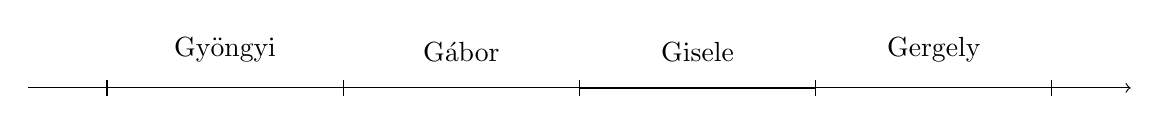
\begin{tikzpicture}
\scaffolding
\draw (2.5,-0.5) node[above=6pt, align=center] {Gyöngyi};
\draw (5.5,-0.5) node[above=6pt, align=center] {Gábor};
\draw (8.5,-0.5) node[above=6pt, align=center] {Gisele};
\draw (11.5,-0.5) node[above=6pt, align=center] {Gergely};
\end{tikzpicture}


\end{frame}







\section{Descriptives}\hypertarget{Descriptives}{}
\longfigure{shares_over_time}{Local and expat managers over time}
\longfigure{CEO_type_by_age}{Founder CEOs are slowly replaced}
\longfigure{CEO_N_histogram}{Firms sometimes have multiple CEOs}
\widefigure{CEO_N_histogram_by}{80 percent of firms have no expat CEO}
\widefigure{CEO_tenure_histogram}{Expat CEOs leave somewhat earlier (median 3 v 4 years)}


\begin{frame}\frametitle{Number of CEO switches}\hypertarget{Number of CEO switches}{}
\begin{tabular}{cll}
\hline \hline
 From &  To domestic & To expat \\
\hline

domestic & 15783 & 1849 \\ 
expat & 2493 & 4774 \\ 
\hline \hline
\end{tabular}




\end{frame}







\section{Research design}\hypertarget{Research design}{}
\begin{frame}\frametitle{Research design}\hypertarget{Research design}{}
\begin{itemize}
\item Take each CEO spell at each firm (e.g., Steve Ballmer, Microsoft, 2000--2014)

\item Exclude founders (e.g., Bill Gates, Microsoft, 1975--1999)

\item For each spell, collect firm-level data for three periods:
\begin{itemize}
\item before (1975--1999)

\item during (2000-2014)

\item after (2015--)
\end{itemize}

\item Comparing these periods, we estimate the impact of a new CEO and whether it is long lasting.


\end{itemize}
\end{frame}



\begin{frame}\frametitle{Manager-level event study}\hypertarget{Manager-level event study}{}
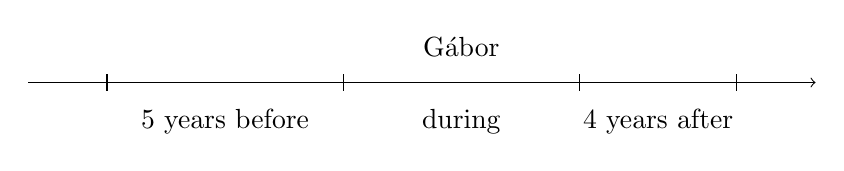
\begin{tikzpicture}
\draw [->] (0,-0.5)--(10,-0.5);
\foreach \x in {1,4,7,9}
\draw(\x cm,3pt - 0.5cm) -- (\x cm, -3pt - 0.5cm);
\draw (2.5,-0.5) node[below=6pt, align=center] {5 years before};
\draw (5.5,-0.5) node[above=6pt, align=center] {Gábor};
\draw (5.5,-0.5) node[below=6pt, align=center] {during};
\draw (8,-0.5) node[below=6pt, align=center] {4 years after};
\end{tikzpicture}


\noindent
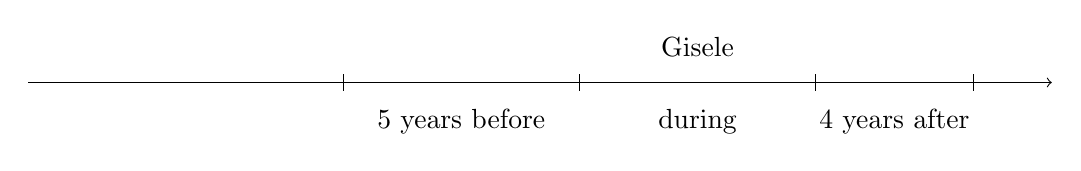
\begin{tikzpicture}
\draw [->] (0,-0.5)--(13,-0.5);
\foreach \x in {4,7,10,12}
\draw(\x cm,3pt - 0.5cm) -- (\x cm, -3pt - 0.5cm);
\draw (5.5,-0.5) node[below=6pt, align=center] {5 years before};
\draw (8.5,-0.5) node[above=6pt, align=center] {Gisele};
\draw (8.5,-0.5) node[below=6pt, align=center] {during};
\draw (11,-0.5) node[below=6pt, align=center] {4 years after};
\end{tikzpicture}


\end{frame}



\begin{frame}\frametitle{Estimating equation}\hypertarget{Estimating equation}{}
$T_{im}\subset [1992,2016]$: tenure of CEO $m$ at firm $i$


$I()$: indicator function


$X_{m}$: expat dummy


\begin{multline*}
Y_{imt} = 
\beta_1 I(t\in T_{im}) + \beta_2 I(t>T_{im}) \\
+\gamma_1 X_m I(t\in T_{im}) + \gamma_2 X_m I(t>T_{im}) \\
+f(\text{age}_{it})
+\mu_{im} + \nu_{st} + \varepsilon_{imt}
\end{multline*}


\end{frame}







\section{Mechanism}\hypertarget{Mechanism}{}


\begin{frame}\frametitle{Three potential benefits}\hypertarget{Three potential benefits}{}
\begin{enumerate}\setcounter{enumi}{0}
\item Better firm-specific skills and loyalty

\item Better general management skills  

\item Reorganization




\end{enumerate}
\end{frame}



\begin{frame}\frametitle{Specific skills}\hypertarget{Specific skills}{}
\begin{tikzpicture}
\scaffolding
\draw [red, very thick](0,0)--(7,0)--(7,3)--(10,3)--(10,0)--(14,0);
\end{tikzpicture}


\end{frame}



\begin{frame}\frametitle{Transferable skills}\hypertarget{Transferable skills}{}
\begin{tikzpicture}
\scaffolding
\draw [red, very thick](0,0)--(7,0)--(7,3)--(14,3);
\end{tikzpicture}


\end{frame}



\begin{frame}\frametitle{Reorganization}\hypertarget{Reorganization}{}
\begin{tikzpicture}
\scaffolding
\draw [red, very thick](0,0)--(4,0)--(4,1)--(7,1)--(7,2)--(10,2)--(10,3)--(14,3);
\end{tikzpicture}


\end{frame}



\begin{frame}\frametitle{Identification concerns}\hypertarget{Identification concerns}{}
\begin{itemize}
\item Reverse causality: Expats come to firms with good prospects.
\begin{itemize}
\item no plausible IV with strong first stage (source countries, EU accession, bilingual schools)
\end{itemize}

\item Omitted variables: Expats are just a signal of strong owner attention.




\end{itemize}
\end{frame}







\section{Estimates}\hypertarget{Estimates}{}
\begin{frame}\frametitle{Foreign firms are better in every respect (OLS estimates)}\hypertarget{Foreign firms are better in every respect (OLS estimates)}{}
\regressiontable{baseline_OLS}


\end{frame}



\begin{frame}\frametitle{Foreign takeover is associated with higher capital intensity, productivity and exporting (firm FE estimates)}\hypertarget{Foreign takeover is associated with higher capital intensity, productivity and exporting (firm FE estimates)}{}
\regressiontable{baseline_FE}


\end{frame}



\begin{frame}\frametitle{Foreign takeover is associated with higher productivity (firm FE estimates on acquisition sample only)}\hypertarget{Foreign takeover is associated with higher productivity (firm FE estimates on acquisition sample only)}{}
\regressiontable{acquisitions_FE}


\end{frame}



\begin{frame}\frametitle{Selection: Better, more global firms receive expat CEOs}\hypertarget{Selection: Better, more global firms receive expat CEOs}{}
\regressiontable{selection}




\end{frame}



\begin{frame}\frametitle{Manager-level estimates on acquisitions sample}\hypertarget{Manager-level estimates on acquisitions sample}{}
\regressiontable{acquisitions}
\end{frame}






\longfigure{acquisitions_lnL_slope}{Local and expat managers reduce employment by same amount}
\longfigure{acquisitions_lnKL_slope}{Capital intensity drops after first expat manager leaves}
\longfigure{acquisitions_lnQL_slope}{Expat managers improve revenue per worker by 15--25 percent}
\longfigure{acquisitions_exporter_slope}{Expat managers increase probability of exporting by 3pp}






\section{Event studies}\hypertarget{Event studies}{}
\longfigure{lnL_event_study}{Expat managers come to somewhat faster growing firms}
\longfigure{lnKL_event_study}{No significant changes in capital per worker}
\longfigure{lnQL_event_study}{Expat managers have persistent effect on revenue per worker}
\longfigure{exporter_event_study}{Expat managers have temporary effect on likelihood of exporting}










\section{Estimates from manager switches}\hypertarget{Estimates from manager switches}{}


\begin{frame}\frametitle{Estimating equation}\hypertarget{Estimating equation}{}
$X_{m}$: manager $m$ is expat 


$X_{m-1}$: previous manager is expat 


omit $t>T_{im}$ years


\begin{multline*}
Y_{imt} = 
\sum_{j=0,1}\sum_{k=0,1} \beta_{jk} I(X_{m-1}=j)I(X_{m}=k)I(t\in T_{im})\\
+f(\text{age}_{it})
+\mu_{im} + \nu_{st} + \varepsilon_{imt}
\end{multline*}


\end{frame}




\longfigure{lnL_tree}{All reorganization results in loss of employment}
\longfigure{lnQL_tree}{Productivity effect of expats remains after they leave}
\longfigure{exporter_tree}{Exporting effect of expats remains after they leave}


\begin{frame}\frametitle{Expats help start exporting, but have limited effect on continuation}\hypertarget{Expats help start exporting, but have limited effect on continuation}{}
\regressiontable{exporter_heterogeneity}


\end{frame}







\section{Interpretation}\hypertarget{Interpretation}{}
\begin{frame}\frametitle{Interpretation}\hypertarget{Interpretation}{}
Three alternative explanations


\begin{enumerate}\setcounter{enumi}{0}
\item Firm-specific skills
\begin{itemize}
\item no substantial heterogeneity with initial firm characteristics other than exporting
\end{itemize}

\item General skills
\begin{itemize}
\item labor productivity improvement has persistent effect
\end{itemize}

\item Reorganization
\begin{itemize}
\item effects of domestic change in management much smaller


\end{itemize}

\end{enumerate}
\end{frame}



\begin{frame}\frametitle{Costs}\hypertarget{Costs}{}
Why does not every firm hire a foreign manager?


\begin{enumerate}\setcounter{enumi}{0}
\item Wages are higher 

\item Search costs are higher

\item Match is less than perfect






\end{enumerate}
\end{frame}







\section{Conclusions}\hypertarget{Conclusions}{}
\begin{frame}\frametitle{Conclusions}\hypertarget{Conclusions}{}
\begin{itemize}
\item Firms with expat managers improve output per worker and enter export markets.

\item Patterns are consistent with a transferable skill interpretation:
\begin{itemize}
\item persistent reorganization

\item technology transfer


\end{itemize}

\end{itemize}
\end{frame}



\begin{frame}\frametitle{Next steps}\hypertarget{Next steps}{}
\begin{itemize}
\item Improve identification with matching.

\item Explore complementarities of expat managers.

\item Explore management team and succession in expat firms.

\item Link to World Management Survey: how do management practices of expats differ?
\end{itemize}
\end{frame}







\end{document}
